\chapter{Introduction}

The goal set forth by this thesis seems ambitious: to introduce a completely new language of uncertainty and information that abstracts away measure theory, probability, etc. and is better primed for computation in estimation and stochastic control algorithms.
Research into this language is well underway in the mathematical community -- this thesis presents it in the context of stochastic dynamical systems, and discusses a methodology for formulating new stochastic estimation and control problems to be solved.

Much discussion in this thesis will be grounded in the classical Kalman filter, as it is a common estimator with which readers will more likely be familiar, and it serves as a good basic starting point for this methodology.
Indeed, the author did in fact get inspiration to study this topic after noticing a connection between propagation of uncertainty in the Kalman filter and the monadic bind operator in functional programming languages. This will be discussed later. While it may seem like we are ``reinventing the wheel'' in that this paper presents what seems to amount to just a new way to program Kalman filters, it must be stressed that the approach presented is hypothesized by the author to generalize to brand new estimators yet to be developed and offers a systematic way to derive them.

This approach to estimator derivation is more than just systematic; there is an aspect which is automatic, in that the user only derives simple elemental building blocks for a representation of uncertainty that they come up with, and more complicated algorithms automatically plumb these blocks together. In a way, this thesis shows that parts of a classical Kalman filter can be automatically derived by a computer.

\todo[inline]{Expand on this thought: at the heart of computer science and engineering fields are two concepts, fundamentally intertwined: abstraction and automation. When we have a repetitive task, a general approach is to find patterns in the repetition, characterize them, and use them to determine a more abstract descriptive language. In this process, the lower level gets an implementation that conforms to an interface to talk with the higher level. This abstraction process can be repeated many times, forming an abstraction ladder, where the highest rung is very general, descriptive, and powerful, and it communicates with the level below it, which propagates all the way to the bottom closest-to-the-metal rung. In this thesis, we use an upcoming mathematical language in a beginning attempt to automate and abstract away the details of deriving estimation schemes for stochastic dynamical systems.}

\section{The Kalman Filter}

\subsection{Definition}

The Kalman filter is a commonly cited estimation routine for tracking uncertain dynamical systems.
The system in question is often modeled in discrete time, and carries a state that is unknown. 

A discrete dynamical system can be abstracted as a point $x\in X$ that evolves in a sequence $\{x_k\}_{k\in \naturals}$.
We call $x_k$ the state at time $k$, which lives in the state space $X$. For the Kalman filter, $X$ is a finite dimensional real-valued vector space $\reals^n$.
Measurements $z\in Z$ are then taken at each time step, where $Z$ is the measurement space. For the Kalman filter, $Z$ is usually taken to be the vector space $\reals^m$. For generality, we will still just refer to the spaces as $X$ and $Z$ respectively, as later on we will discuss generalizing these beyond vector spaces.

The mappings are linear with additive Gaussian noise. The dynamics and measurement models respectively are given by
\begin{equation}
	\label{kalman-filter-models}
	\begin{aligned}
		x &= Fx_- + w,\ w\sim\gaussian(0,Q)\\
		y &= Hx + v,\ v\sim\gaussian(0,R)
	\end{aligned}
\end{equation}
where $F:X\rightarrow X$, $H:X\rightarrow Z$, $Q\in \symmetric^X_+$, and $R\in\symmetric^Z_+$.
For simplicity, we omit the explicit references to time dependency and drop the subscripts for the time sequence.
Here we really only consider a single time step $k$ within the algorithm, as the algorithm is recursively looped and each step is implemented in the same way. If a variable has no subscript, it can be assumed that it draws from time step $k$. If it has the subscript ``$-$'', then it comes from the $k-1$ time step.

%We switched the notion from additive noise to a formal sum. This is more a change in mindset and doesn't affect the outcome. In traditional texts, the equation $y = Hx + v,\ v\sim \gaussian(0,R)$ implies that the measurement model is an affine mapping, with an additive vector $v$ that gets drawn from a Gaussian distribution. Here, however, we add the distribution directly in a \emph{formal} sum in what we call a decorated linar map\cite{extended-gaussian}. The plus sign does not indicate that the distribution is literally added to the vector, which would be impossible, but simply that there is uncertainty attached to the model. 

Remark: $Q$ and $R$ are not strictly positive-definite, but they are relaxed to being positive semi-definite. This allows for the case where there actually is certainty, be it complete certainty or certainty within a subspace. This can also be extended to uninformative priors, again as in \cite{extended-gaussian}.

Remark: In traditional treatments of the Kalman filter, $\{w_k\}_k$ and $\{v_k\}_k$ are viewed as Gaussian processes, meaning the entire history of each sequence is jointly sampled from a single probability space. This means that correlation between different time steps need to be taken into consideration. It is assumed that disturbances are Markov, meaning that each $w_k$ is independent from $w_j$ at another timestep $j$, or in other words that $E(w_kw_j^T) = 0$ for $k\neq j$. In our basic categorical treatment of filtering, this Markovian aspect will be implied, as all kernels are Markov kernels. The only way to get autocorrelation in a process will be to explicitly specify that a distribution is a member of a joint space. When we consider Markov categories as applied to stochastic processes, things may change.

Our posterior knowledge of the state is characterized by a Gaussian uncertainty.
Thus at the current time step, the posterior knowledge from the prievious timestep is given as $\gaussian(\hat{x}_-, \hat{P}_-)$.
This is pushed through the dynamic model in Equation \ref{kalman-filter-model} to get the prior belief $\gaussian(\bar{x}, \bar{P})$ of the state at the current time step, with
\begin{align}
	\label{kalman-filter-dynamics-push}
	\bar{x} &= F\hat{x}_-\\
	\bar{P} &= F\hat{P}_- F^T + Q
\end{align}
Further, this then gets propagated to our belief on where the measurement will fall, $\gaussian(\bar{z}, S)$ with
\begin{align}
	\label{kalman-filter-measurement-push}
	\bar{z} &= H\bar{x}\\
	S &= H\bar{P} H^T + R
\end{align}
our belief on where the measurement will fall, $\gaussian(\bar{z}, S)$ with

This next part we will present in a way that's slightly rearranged from common texts, but which sets the stage or further generalizing the filter.
In particular, typically a measurement error is defined as $\tilde{y} = z - \bar{z}$, but we define the following:

\begin{align}
	K &= \bar{P}H^T S^{-1}\\
	\tilde{x} &= \bar{x} - K\bar{z}
\end{align}

We then get our posterior estimate

\begin{align}
	\hat{x} = Kz + \tilde{x} \\
	\hat{P} = (I-KH)\bar{P}
\end{align}


\subsection{Recasting the Datatypes}

Random variables are often described as variables that take on values (ie.\ real numbers) in a random fashion.
There is a frequentist sort of nature to this description, as if a random variable is a number that changes its value every time you look at it.

\todo[inline]{Discuss interpretations and formalizations of random variables. In particular, the formalization that a random variable is a \emph{function} from a probability space taking on values in a state space is just so clunky to work with. It opens up ambiguities, for instance in the ASE department's discussion of MMSE, that are so confusing.}

There is an alternative viewpoint: what is often called the Bayesian view of probability.
It states that probability (of an event) is simply a measure of our belief in a state, or more specifically the amount we believe that a state will fall into that event.
We wish to take this viewpoint and run with it, generalizing into many different ways of characterizing our belief or information on the state of a system.

The parameterization of our knowledge of the state lives in a separate space from the state itself.
While the system itself has a state $x\in X$, our knowledge of it, characterized by a Gaussian distribution, has a parameterization $(x,P)\in X\times \symmetric^X_+$.
To simplify our language, we wish to define a space in which each element is a distribution. For the Gaussian case, we shall define $\gaussian(X)$ to be the space of Gaussian distributions on $X$, where $X$ is some finite dimensional real valued vector space $X=\reals^n$. This changes our perspective and modifies our notation: previously, we would view the notation $x\in X,\ x\sim \gaussian(\hat{x}, P)$ to mean ``$x$ is a system state living in the state space $X$, but we don't know where it is. Our knowledge of where it might be is given by the distribution $\gaussian(\hat{x}, P)$, and observing it directly would be akin to sampling the probability distribution''. Under this new construction, we could change the notation to $x\in \gaussian X,\ x = \gaussian(\hat{x}, P)$.
The change in notation is subtle, but the difference in interpretation is significant. This new notation would be interepreted as ``$x$ \emph{is} our knowledge of where the system state may lie, and it lives in the collection of Gaussian distributions on $X$. $x$ \emph{is equal to} such and such distribution.''\todo{Write this better}.

For practicality, we parameterize. A class of anything\todo{write this better} is isomorphic to its parameterization, and in the case of Gaussians each distribution is fully parameterized by its mean and covariance. Thus, we have $\gaussian X \cong X\times \symmetric^X_+$, and for purposes of discussion they can be considered equivalent.

Note that this forms a type level mapping $\gaussian : \FinVect \rightarrow \gausscat$ with

\begin{equation}
    \gaussian : X \mapsto \{(x,P) : x\in X, P \in \symmetric^X_+\}
\end{equation}

This is a functor, meaning it also maps mappings.

\subsection{The kernels}

Given that we have gotten rid of sampling from distributions, we must change the way we notate the models in \ref{kalman-models}. We also wish to change our perspective, similar to section \ref{datatypes}.

Consider a generic mapping of the same type in Equations \ref{kalman-models}.

\begin{gather}
	\label{generic-mapping}
	y = Hx + v
\end{gather}

Where $x\in X$, $H:X\rightarrow Y$, $v\sim \gaussian(\hat{v}, Q)$.
We wish to recast our treatment of dynamics and measurement models from equations to functions. One important reason for this is that in a functional programming language, functions are data, and a function is an element of a datatype. This becomes much more handy for computation than an equation, which is slightly more unweildy to carry around (we don't really assign variable names to an equation but we do to functions), and equations represent relations which are slightly less compatible with computation than functions are.

Thus we would like to say that Equation \ref{generic-mapping} is represented by a function $h$.
Given a traditional view of random variables, one could think of $h$ in two ways.

If random variables are thought of as functions from a probability space, say $x:(\Omega,\mathcal{F}, P)\rightarrow X$ and $v:(\Omega,\mathcal{F}, P)\rightarrow Y$, then $h$ is a functional operator built up from an induced algebra on functions. In particular, the application $Hx$ is actually a function composition $H\circ x : \Omega \rightarrow X \rightarrow Y$. The addition $Hx + v$ refers to the addition of the functions $H\circ x$ and $v$, where function addition is defined as being induced from the addition of their results. Thus, with this viewpoint, we define $h$ as a functional mapping $h:(\Omega\rightarrow X) \rightarrow (\Omega\rightarrow Y)$ where $h[x](\omega) = H(x(\omega)) + v(\omega)$. When discussing the probability distributions that random variables take, these are defined through pushforward measures. The probability distribution of $x$ is defined as $x^*(P)$, and thus the distribution on $y$ is $(h[x])^*(P)$.

An frequentist viewpoint is to think of random variables as \emph{values} that we do not immediately know. With this view, we would say $x\in X$, $H:X\rightarrow Y$, $v\in Y$, where $v$ is a value that gets added to the \emph{value} $Hx$ using the algebraic structure on elements in $Y$. The true value of these quantities is unknown, thus we think of them as being sampled from their respective distributions. We then give them the treatment of how algebraically manipulating values with uncertainty affects their underlying probability distribution.

We wish to be a bit more direct in our definitions as we did in section \ref{above}. The important aspects of stochastic kernels is how they affect probability distributions, so the fundamental unit in this thesis from hereon out is a mapping on spaces of distributions. Thus for Kalman filters, we recast Equation \ref{generic-mapping} as a function
\begin{equation}
	h:\gaussian X\xrightarrow[v\sim\gaussian(\hat{v},Q)]{y = Hx + v} \gaussian Y
\end{equation}
We may shorten this notation to $h:\gaussian X \xrightarrow[\gaussian(\hat{v},Q)]{H} \gaussian Y$ or simply to $h = (H, \gaussian(\hat{v},Q))$.
Seeing how the means and covariances get mapped through models in Equations \ref{kalman-filter-dynamics-push} and \ref{kalman-filter-measurement-push}, we will define such a map as

\begin{equation}
	\label{gaussian-map}
	h:\gaussian X\ni (\hat{x},P) \xmapsto[\gaussian(\hat{v}, Q)]{H} (H\hat{x} + \hat{v}, HPH^T + Q) \in \gaussian Y
\end{equation}

From this, we can immediately rewrite much of the Kalman filter in a more compact form. 

Say that $x_- = (\hat{x}_-, \hat{P}_-)\in \gaussian X$ is given, and we have dynamics model $f = (F,\gaussian(0,Q)):\gaussian X \rightarrow \gaussian X$ and measurement model $h = (H,\gaussian(0,R))$ that map $x$ according to Equation \ref{gaussian-map}. If we pattern match $(\bar{x}, \bar{P}) = f(x_-)$ and $(\bar{z}, S) = h(f(x_-))$, then the Bayesian inversion of $h$ is given by
\begin{equation}
    \label{kalman-dagger}
    h^\dagger = (K, \gaussian(\tilde{x}, \hat{P})) : \gaussian Y\rightarrow \gaussian X
\end{equation}
where $K$, $\tilde{x}$, and $\hat{P}$ are given by Equations \ref{kalman-gain}, \ref{expected-residual}, and \ref{updated-covariance} respectively. This gets applied to a given measurement $z = (z,0)\in \gaussian{Z}$ as $x = h^\dagger(z)$.

There are actually two more kernels hidden here, that we will develop now just for completeness. To set the stage, consider a set $X$ and an element $x\in X$. Also consider the singleton set, $\singletonset$, which has just one element that we call ``$\cdot$''. A function $f:\singletonset\rightarrow X$ has only the single element $\cdot$ in its domain, thus its range in $X$ also consists of a single element. This means that the hom set $\Set(\singletonset, X)$ is equivalent to $X$ itself, ie.\ that picking an element $x\in X$ is equivalent to picking a function $x:\singletonset \rightarrow X$. Mapping an element $x\in X$ through a function $f:X\rightarrow Y$ as $y=f(x)$ is then equivalent to composing functions $f\circ x:\singletonset\rightarrow X\rightarrow Y$ as this yields simply another function $f\circ x = y :\singletonset\rightarrow Y$.

We can do the same thing for distributions. The trivial vector space, $\reals^0$, has a single element, $0$. This single element can also be viewed as $[]$, the empty list of length 0. For any $\reals^n$ there is only one function $F:\reals^0\rightarrow \reals^n$ which maps to $0\in\reals^n$ and has an empty matrix representation $[]\in \reals^{n\times 0}$. The space of distributions $\gaussian \reals^0$ has a single distribution $([], [])$ whose mean is an empty $\reals^0$ vector and covariance is an empty PSD matrix $0\in\symmetric^0_+$. Note that although the covariacne is an empty matrix, its scalar value is 0 and is thus PSD. This represents a dirac distribution centered around the degenerate origin. A kernel then is a map $\gaussian \reals^0 \xrightarrow[\gaussian(\hat{x},P)]{[]}\gaussian \reals^n$ that picks a single distribution in $\gaussian\reals^n$ based on the mapping in Equation \ref{gaussian-map}: the mean is $0^{n\times 0}0^0 + \hat{x}$ and the covariance is $0^{n\times 0}0^{0\times 0}(0^{n\times 0})^T + P$. From this point forward in the thesis, we will treat distributions as functions coming out of the unit space of a single degenerate distribution. In practice, depending on the programming language used, it might be easier to pick one representation or another.

Note the similarities but also the distinction between this equivalence and the measure theoretic treatement of random variables. In measure theory, a random variable was thought of as an element $x\in X$ with some mysterious uncertainty to it, but behind the scenes it was actually a mapping from a sample space $x:\Omega \rightarrow X$ that pushed a probability measure through it $P \mapsto x^*(P)$. A deterministic function $f:X\rightarrow Y$ was treated as being applied to $x$ in $y = f(x)$, when in reality behind the scenes it was composed as $y = f\circ x : \Omega \xrightarrow{x} X \xrightarrow{f} Y$. This would simply yield a new random variable $y:\Omega\rightarrow Y$ with its own pushforward. Nondeterministic Markov kernels $p(y|x)$ required more complicated considerations and further definitions such as conditioning. In our treatment, we treat random variables as functions $x:\probfunc \singletonset \rightarrow \probfunc X$, when equivalently it could be an element $x\in\probfunc X$. We can map through \emph{any} non-deterministic kernel $f:\probfunc X \rightarrow \probfunc Y$, either as an element $x\mapsto f(x) = y$ or as a composition $y = f\circ x : \probfunc\singletonset \xrightarrow{x} X \xrightarrow{f} Y$ to yield a new distribution function $y:\probfunc\singletonset \rightarrow \probfunc Y$. Depending on the programming style and language chosen, one characterization or the other may be ideal, but here in this thesis we consider distributions to be functions from the singleton.

Given this treatment, the Kalman filter can be rewritten yet again: given the following 3 kernels
\begin{equation}
    \label{kalman-mappings}
    h\circ f\circ x:
    ([],[])
    \xmapsto[\gaussian(\hat{x}_-, \hat{P}_-)]{[]}
    \gaussian(\hat{x}_-, \hat{P}_-)
    \xmapsto[\gaussian(0,Q)]{F}
    \gaussian(\bar{x}, \bar{P})
    \xmapsto[\gaussian(0,R)]{H}
    \gaussian(\bar{z}, S)
\end{equation}
the Bayesian inversion of $h$ with respect to $f\circ x$ is $h^\dagger$ as given in Equation \ref{kalman-dagger}. Given the kernel $z : ([],[])\xmapsto[\gaussian(z,0)]{[]} \gaussian(z,0)$, we apply it through the Bayesian inversion to get $x = h^\dagger\circ z$.

This begs the question: we have 3 kernels that we combine in some way to get the Bayesian inversion $h^\dagger$. This isn't just blind composition either: we take the prior $\gaussian(\bar{x}, \bar{P})$, and before we send it on its way through $h$, we make a copy of it, and use those results along with the results after mapping through $h$ to generate $h^\dagger$. Is there a systematic way of doing this without deriving the Kalman gain and covariance update by hand? Can we avoid using Gaussian PDFs in this derivation? Can we generalize this process to other types of kernels or distributions? This is the thesis of my thesis.\todo{I wrote this at 12:30 AM, obviously}

\subsection{Assumptions}

Several assumptions are made in the structure of the Kalman filter. In the quest for generalization and in search of a \emph{prejudice free} filter \cite{some-moriba-paper}, we enumerate assumptions and generalizations that this framework can potentially strip away.

\paragraph{State Space}

Systems modeled for the Kalman filter have states that live in a finite dimensional real-valued vector space. Many interesting systems, however, live in much more general spaces that can be hard to characterize in a computer program. \todo[inline]{Put this somewhere: We believe that the framework presented could potentially offer a systematic way to represent state spaces. Talk about procedurally generated algorithms somewhere.} Many systems would be more accurately represented as a Hilbert or Banach space, Riemannian manifold, Lie group, finite space, topological space, general measure space, or something else. In taking a categorical approach to dynamical systems, we generalize $X$ to be \emph{any} kind of state space.

\paragraph{Uncertainty Representation}

Uncertainty in the state is taken to be a multivariate Gaussian probability distribution. Beyond the fact that generalizations in the type of state space warrant alternate considerations for probability, we wish to generalize notions of uncertainty beyond probability density functions and even beyond probability itself. Common practices involve treating uncertainty as being a distribution with a PDF, but in a measure theoretic context there exist probability spaces whose probability measure is not differentiable or ``nice looking'' in a smooth or continuous sense. Further, there are representations that go beyond probability even: we could wish to represent our knowledge of system state with \emph{possibility}, where at a given time we know the system lies in a certain region, but we know nothing of where in the region it lies. There are more exotic representations of uncertainty, such as outer probability measures \cite{houssineau} or higher order probability \cite{some moriba paper} that could potentially fit into this framework. In total, we wish to abstract $\gaussian X$ into $\probfunc X$, which represents a generic class of information distributions on $X$. For instance, we could have $\probfunc(X) = 2^X$ the power set of $X$. An element $x_0\in 2^X$ is merely a subset of $X$, and thus would be a fine representation for an initial state possibility distribution for the system. Another well known example is the Giry monad $\giry$ on a measurable space $X$, which is the class of all probability measures on $X$ endowed with its own induced sigma algebra.

Remark: there is some practicality to note. Ultimately, $\probfunc$ will be constructed as a datatype mapping, or $\probfunc(X)$ will be explicitly constructed as a datatype itself. Not all information representations, for instance general probability measures, can be practically constructed as a datatype.

\paragraph{Kernels}

\todo[inline]{This will be about the assumptions made in the kernels. They're decorated linear maps, or can be thought of as linear maps with additive gaussean noise. We want to generalize to any generic mapping between classes of knowledge representaitons.}

We can make similar generalizations that we made above. In the Kalman filter, a kernel is thought of as a linear map with additive noise, through which we defined a map $f:\gaussian X\rightarrow \gaussian Y$. Imposed on the underlying maps were a restrictive linear structure, which made them well defined on a restricted class of probability distributions. If we strip away as many assumptions as we can, while keeping the notion that we are mapping between classes of distributions, then we are left with kernels $f:\probfunc X \rightarrow \probfunc Y$, that is, a generic map between generic families of probability distributions over generic spaces. Coming back to the questions from Section \ref{kalman-filter-kernels}, the reformulation of the Kalman filter therein allows us to generalize to a generic formulation to a generic filter:

Say a system has a state space $X$, where $X$ can be a finite dimensional vector space, Hilbert space, manifold, topological space, or any other kind of structure. We take measurements in a space $Y$, which also can have some exotic structure, and $\probfunc X$ and $\probfunc Y$ are classes of uncertainty distributions on $X$ and $Y$ respectively. $\probfunc X$ can be the class of subsets (aka the powerset), collection of probability measures, convexly weighted finite subsets, Gaussian distributions, whatever. We have some prior knowledge of a system state, $x\in \probfunc X$, a dynamics model $f:\probfunc X\rightarrow \probfunc X$, and a measurement model $h:\probfunc X\rightarrow \probfunc Z$. What structures do these things need at an absolute minimum for us to do filtering? Can we compose them in a way to automatically form a Bayesian inversion $h^\dagger : \probfunc Z\rightarrow \probfunc X$ through which we can feed our measurement and get out an updated posterior? If this can be achieved through function composition, then this can be automated. We can write a computer program into which we feed dynamics and measurement models, and from which we recieve update laws. This could greatly reduce the amount of analysis required to find new estimation algorithms. Further, the door could be opened for more algorithms involving stochastic dynamical systems to be composed in such a fashion.

The answer to the first question in the previous paragraph: what's the minimal structure the kernels need for filtering, is known. The kernels need to form a Markov category with conditionals. This will be explored in Section \ref{categories}. And the second question is also answered here. We indeed can write filtering programs at a higher level: not just programs that take in states and give estimates, but programs that take in models and give update laws. We will discuss the basics behind a framework in Section \ref{abstract programming}.

\section{Abstract Programming}
\todo[inline]{Write this. Make it general, Describe the figure}

This thesis presents a framework for programming estimation algorithms in a way that splits the high level structure of for instance a recursive filter, from the low level implementation of uncertainty representation. This framework works in such a way that code from the high level gets inherited by the low level. In the case of the Kalman filter, the abstract side of the framework involves high level plumbing and composing of generic kernels to create an update law. 
\todo[inline]{Chapter 2, background, will have an abstract programming section that will go more in-depth. It will talk about the interface between the two levels which provides the protocol aka the categorical structure in which kernels should conform, so that low level and high level can talk. We won't talk about the interface here.}
\todo[inline]{There are further thoughts for the framework. In detail, the Kalman filter code contains 4 parts: The high level recursive filter algorithm, the low level Gaussian kernel implementation, the interface that tells the low level which methods to implement and provides those methods to the high level, and the implementation code that says "f has these matrices, h has those matrices, here's my prior, and here are my measurements." Put this in a further section}

The low level involves creating a datatype to represent Gaussian transition kernels. 
\todo[inline]{Continue this thought....}

\begin{table}[]
    \centering
    \begin{tabular}{ccc}
	Abstract Algorithms &               & Concrete Representations \\ \hline
	Recursive Estimator & $\Rightarrow$ & Gaussians               
    \end{tabular}
\end{table}

\begin{table}[]
\centering
\resizebox{\textwidth}{!}{%
\begin{tabular}{rcl}
Abstract Algorithms &  & Concrete Representations \\ \hline
Recursive Estimator &  & Gaussians \\
Batch Estimator &  & Unscented Transforms \\
Stochastic Control Problem Formulation &  & Gaussian Mixtures \\
Causal Inference & $\Rightarrow$ & FinStoch \\
Model Estimation &  & Particles \\
&  & Unscented Mixtures \\
&  & Higher Order Uncertainty \\
&  & Possibility \\
&  & Linear Approximated Gaussians
\end{tabular}%
}
\end{table}

\begin{figure}[htb]
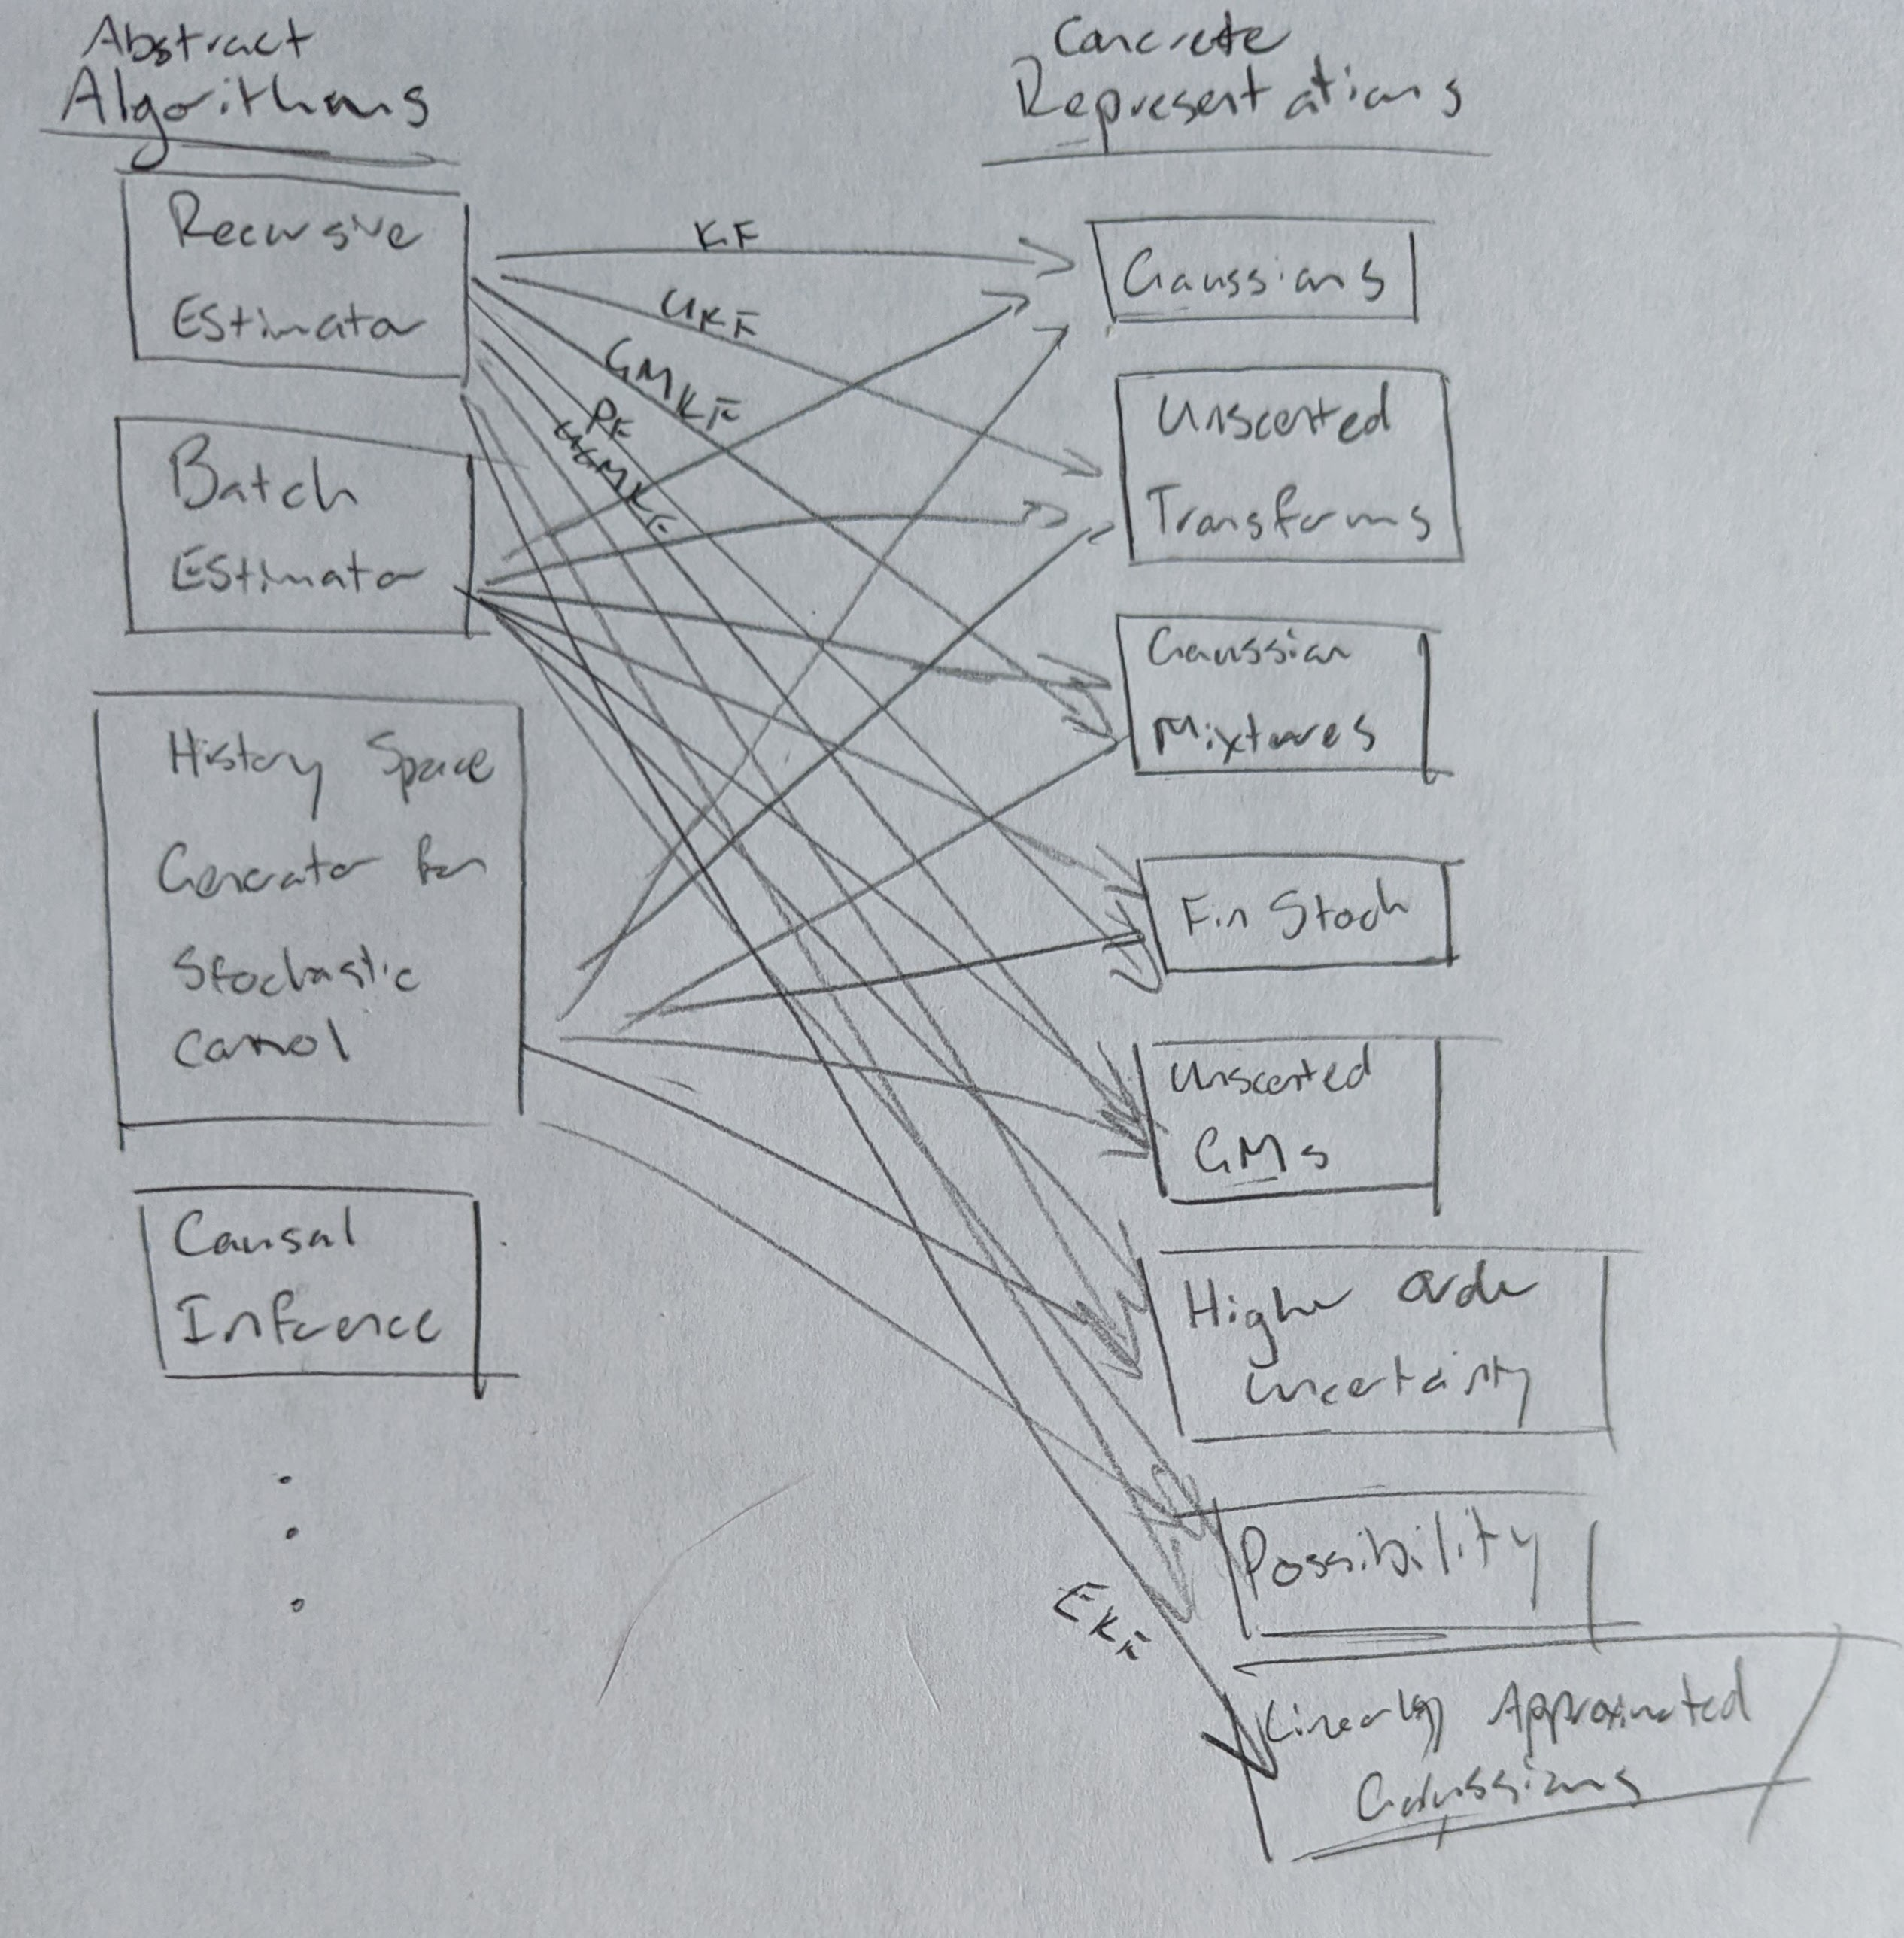
\includegraphics[width=0.5\textwidth]{algorithm-inheritance}
\caption{}
\label{fig:algorithm-inheritance}
\end{figure}

\section{Looking at Markov Transition Kernels}
\todo[inline]{Eliminate this or incorporate into previous}

There is often some conflation between conditionals and transition kernels.
In a way, they are often considered to be developments from the basics of probability.
This stems from the fact that in traditional probability theory, the probability distribution or probability measure is the fundamental notion from which all other definitions and developments are derived.
Similar to how in categorical thinking, where the perspective is switched from sets being fundamental to functions being fundamental, we want to change lenses away from distributions and onto kernels as being the most elemental construction from which distributions, statistics, and algorithms are derived. 
Of course, it significantly helps us in our understanding if we already have some insight into a traditional measure-theoretic way of thinking about probability, but this is not totally necessary.
It more serves as a grounding point, similar to when learning category theory -- it helps greatly to already be familiar with sets+functions, vector spaces+linear maps, topoligical spaces+continuous maps, groups+group homomorphisms, and so on so that we have a \emph{context} for where categories are really useful as a language to describe stuff instead of only this abstract notion of arrows and objects and categories of categories.

Before giving a formal definition of categories, we should just mention for the familiarity of the reader that a category is made of arrows called \emph{morphisms} that are useful in describing mappings between spaces. In categorical probability, these morphisms can describe \emph{mappings that behave like Markov transition kernels}.

But what exactly is a transition kernel?
Intuition would say that it is a mapping between distributions, but there is a bit more nuance than that. ** Add some text to introduce these equations **

\todo[inline]{List all the different types of transition kernels you've seen and talk about their differences and similarities. The goal here is to show how they can be unified into the categorical framework.}

\begin{equation}
\label{traditional-gaussian-model}
\begin{gathered}
    y = Fx + w \\
    w \sim \gaussian(\bar{w}, R)
\end{gathered}
\end{equation}

\begin{equation}
    \begin{aligned}
	y = f(x,w)
    \end{aligned}
\end{equation}
\todo{Talk about how this has randomness pushback}
\todo[inline]{Talk about how the frequentist view of these kernels sees that w gets sampled in the instant that y gets evaluated, and acts as a modifier to Fx. We want to change this to a Bayesian view, where F evaluates by taking in an x and returning a distribution. A p(y|x) kind of thing. The problem is that bar notation, tilde notation, and distributions in the Bayesian context SUCK (** this is your personal view point; be more ``diplomatic''; explain why is that **). This is where the functors come in.}

One minor change to our language that can have significant impact is in the recasting of equations into functions\todo{expand on this}.

\section{The Signature of Kernels}
\label{sec:kernel-signature}

One confusing aspect of Markov transition kernels is their signature. 
Standard texts describe the a kernel as the following:

\todo{markov kernel definition}

The important bit is in the partial application: parameterizing $\kappa$ with $x$, the function $\kappa(\cdot, x)$ is a probability measure from $\mathcal{B} \rightarrow [0,1]$ and parameterizing with $B\in \mathcal{B}$, the function $\kappa(B,\cdot)$ is a \emph{mapping whose domain is $X$}.
This is important: $\kappa$ does not input values of distributions, but rather values of state.
This is evident in the confusing bar notation: $p(y|x)$ reads as ``$p$ of $y$ given $x$".
In other words, the transition kernel gives a distribution on $Y$ given a fixed value of $x\in X$.

Using Currying ie.\ partial application\todo{expand on this?}, we can rewrite this signature. 
Since $\giry Y$ is defined to be the collection of distributions on $Y$, then there is an equivalence between $\kappa : \mathcal{B} \times X \rightarrow [0,1]$ and $\kappa : X \rightarrow \giry Y$.

We can give the same treatment to Gaussian models of the form in Equation \ref{eq:traditional-gaussian-model} in Kalman filters, which are also just Markov kernels. The maps just happen to be linear and the distributions gaussian.
While we treat $x$ as a random variable in $y = Fx + w$, the $F$ does not take in random variables.
It takes plain old vectors.
We had to do the work of figuring out how to propagate covariance through $F$.
Further, \ref{eq:traditional-gaussian-model} injects its own distribution into the codomain through $w$.

\todo[inline]{Say something about frequentist statistics}

Using a similar approach to above, let's recast the signature into the new datatype.

\todo[inline]{Talk about how the kernel $\kappa$ has a signature $\mathcal{B}\times X \rightarrow [0,1]$, but we can equivalently formulate it as $\kappa : X \rightarrow \mathcal{P} Y$}

\section{Functional Programming}
\subsection{Higher Order Functions}

A powerful feature of the functional programming paradigm and the first class citizenship of functions is that 

\subsection{Higher Order Types and Type Functions}
\subsection{Typeclasses and Abstract Base Classes}

